\documentclass[../main.tex]{subfiles}
\graphicspath{{\subfix{../images/}}}
\begin{document}
	
	\chapter{Theory}
	\section{Charged-coupled devices (CCDs)}
	A charge-coupled device (CCD), is a solid state image sensor used to detect light. It is an integrated circuit that is essentially an array of metal-oxide semiconductor (MOS) capacitors (MOSCAP) representing the pixels, forming a photoactive region of silicon. In addition the CCD also consists of a shift register to transfer the accumulated charge, that will be interpreted as an image. 
	
	\subsection{Semiconductors}
	Silicon is a semiconductor. A semiconductor is a type of solid state material, which is neither a conductor or an insulator. This distinction between insulators and conductors is defined from the difference in the density of states at the chemical potential at a temperature of $0K$\cite{solidstatephysicsbook}. For metals we have a finite density of states, and otherwise it is an insulator or a semiconductor. A semiconductor is, in addition to the former, a material for which the band gap between the highest occupied states in the valence band, and the lowest unoccupied states in the conduction band, is sufficiently small to thermally excite electrons across the gap. This gap is usually in the order of magnitude of a few electron volts. 
	
	A semiconductor is by definition a solid for which the chemical potential at absolute zero is placed at an energy such that the density of states is zero. This is around the center of the band gap. At finite temperature, some of the electrons from the valence band are thermally excited into the conduction band. This leaves behind so called holes in the valence band. Holes are simply a convenient way to describe the absence of electrons, allowing for us to treat them as positively charged quasiparticles. The movement of electrons through the valence band is permitted by the presence of holes, which in turn can be seen oppositely, as the movement of a hole in the opposite direction. Holes are hence chrage carriers in the valence band allowing conduction. We call electrons and holes 'carriers', and the concentration of carriers are in part what determines the conduction properties of a material. 
	
	The concentration of carriers in an intrinsic semiconductor, that is one which is pure, is too low to give an appreciable contribution to conduction properties. A way to circumvent this problem is by doping the semiconductor. This is a process in which we introduce impurities in the solid. These impurities, also called dopants, can either function as donors, also called \textbf{n doping}, in which they are able to donate electrons to the solid, or as acceptors, also called \textbf{p doping}, in which they take electrons in turn producing a hole. N dopants are chosen such that, at not too high temperatures, the states lie just below the conduction band minimum (CBM), while the p dopant states are just above the valence band maximum (VBM). 
	
	\subsection{The pn-junction} 
	The MOSCAP is an example of a practical technological application of semiconductor physics that is based on the working principles of the pn-junction. The pn-junction is the boundary between regions of a p- and n-doped semiconductor, and is achieved by doping inhomogenously. In the n-doped region most donors are ionized, and the majority carriers are electrons, while in the p-doped region, acceptors are negatively charged, and the majority carriers are holes. 
	
	As the two regions are joined, electrons diffuse into the p-region and holes into the n-region. This leads to recombination of electron-hole pairs as they meet. This gives rise to a region at the boundary, of immobile acceptors and donors, whose charge is not compensated by mobile charged carriers. We call this site the \textbf{depletion layer}. The thickness of this layer is around $0.1$ to $1 \mu$m \cite{solidstatephysicsbook}. An electric field is formed due to the presence of the immobile ionized donors and acceptors. The electric field points from the, now net-positively charged n-region into the negatively charged p-region, presenting as an obstacle for holes to move from the p-region to the n-region. The depletion layer widens, and the field increases, until an equilibrium between the electromagnetic and diffusion forces is reached. There is hence a \textbf{diffusion current} across the region for those carriers with enoguh energy to overcome the opposing eletric field, and a \textbf{drift current} due to the presence of the same field. The chemical potential in the p-doped region lies close to the VBM, and in the n-doped region is close to the CBM, as can be seen via an argument on charge neutrality. However, if we apply a voltage across the depletion layer the equillibrium between these currents is broken such that a net current\cite{solidstatephysicsbook} is produced
	\begin{equation}
		I = I_\text{diffusion} - I_\text{drift} = I_0\left(e^{eV/k_BT}-1\right)
	\end{equation}
	Where $V$ is the so-called \textbf{bias voltage}. This bias voltage is essentially what lets the diode function as a valve for the current. 
	
	\subsection{The MOS capacitor}
	The MOSCAP is a part of the so-called MOSFET structure. A MOSFET is a type of transistor made from the principle of the pn-junction, and is usually constructed from silicon. A MOSCAP is constructed by forming a layer of silicon-dioxide on top of a p-doped semiconductor. On top of this metal or polycrystalline silicon is deposited functioning as an electrode, aslo called the gate, which is the source of the bias voltage. Silicon dioxide is a dielectric insulator, so this construction is akin to a planar capacitor. See figure \ref{fig:mosfet}.
	
	\begin{figure}[h!]
		\centering
		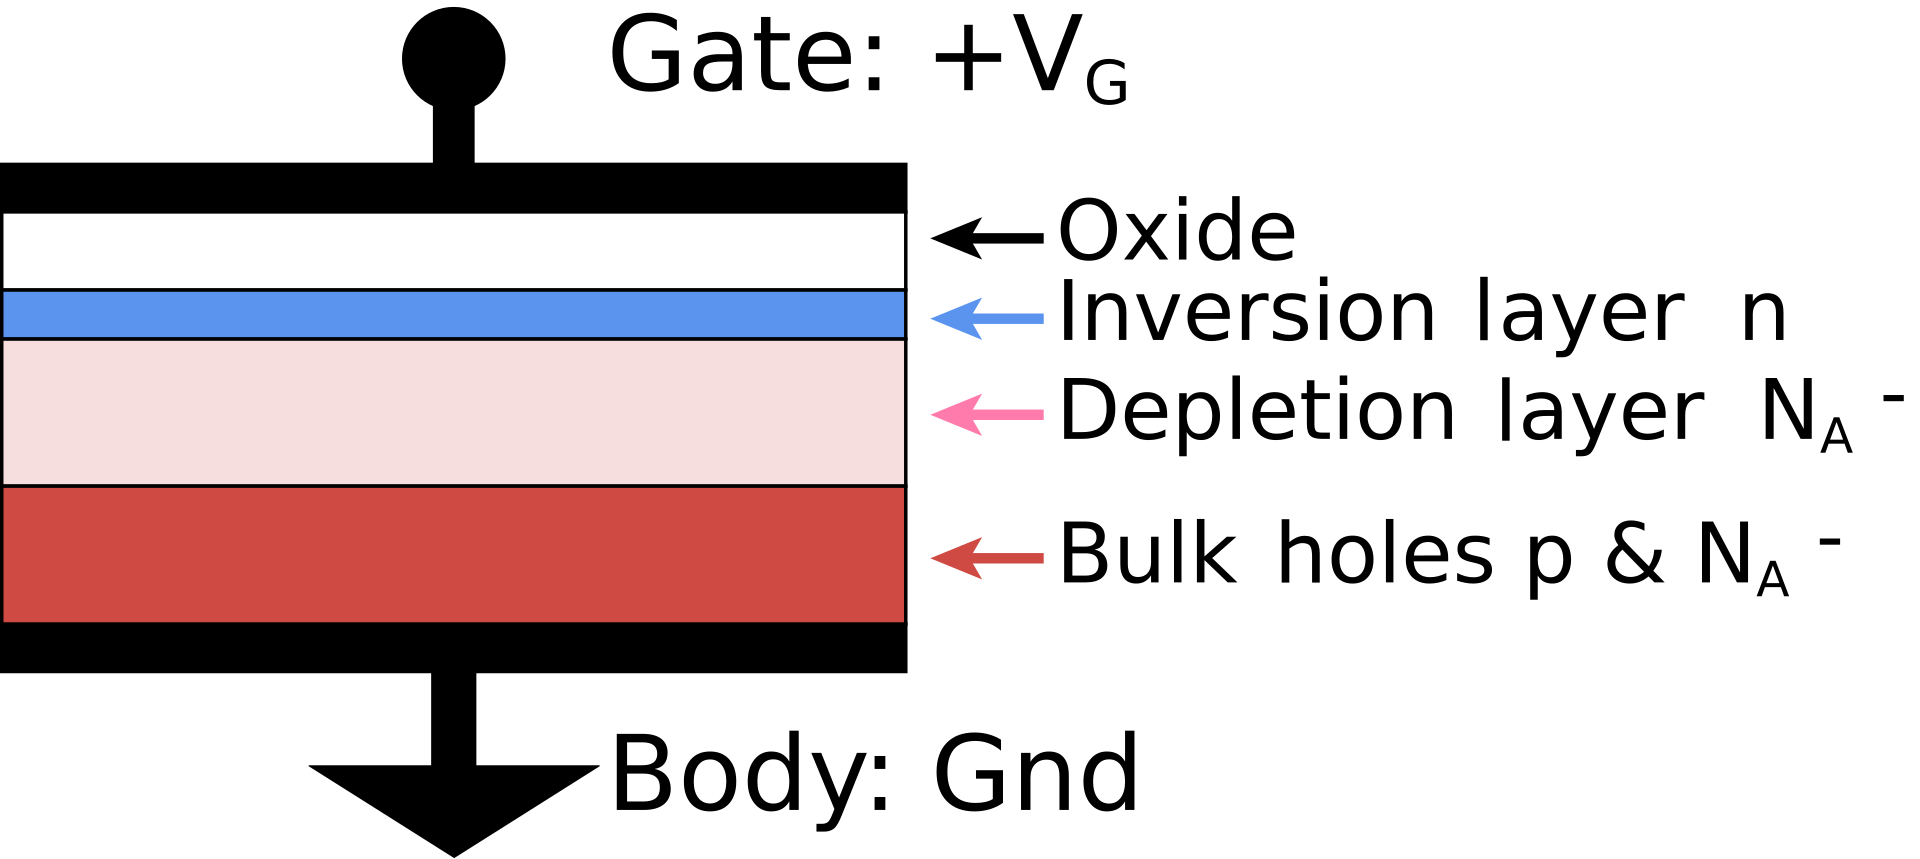
\includegraphics[width=0.5\textwidth]{MOS_Capacitor.png}
		\caption{A MOS capacitor (MOSCAP). Image by Brews ohare — Own work. Licensed under CC BY-SA 4.0, via Wikimedia Commons.
		}
		\label{fig:mosfet}
	\end{figure}
	When a voltage is applied to the gate, holes in the body, the p-type substrate, will be repelled, and minority electrons will be attracted, generating a depletion layer unerneath the oxide layer. If the voltage is great enough, enough electrons will be attracted, and electrons become the majority carriers, forming an n-type region. We call this layer an \textbf{inversion layer}. The threshold voltage at which this happens is an important parameter. It is defined as that voltage, at which the density of the electrons in the inversion layer is the same as that of the density of holes in the p-type substrate. 
	
	If in addition, two so-called \textbf{terminals} are included on either side of the body, consisting of n-doped regions (opposite type compared to the body type), the source and the drain, we call the structure a \textbf{MOSFET}. In the case of a p-type (n-type) body, and two n-type (p-type) terminals, we denote it an nMOSFET (pMOSFET)  or n-channel MOSFET. This makes up two pn-junctions. As voltage is applied to the gate and the inversion layer forms, a channel is formed that will allow current flow. The higher the voltage the greater the electron carrier density, and hence the greater the current flow between the two terminals. Transistors either amplify or switch electronic signals, and are essential building blocks in electronics. 
	
	\subsection{CCD charge generation}
	Before exposure of the CCD the MOSCAPs in the array are biased into the depletion region, thus having not formed the inversion layer at this point. The gate is then biased positively (in n-channel MOSCAPS) above the threshold for inversion, creating an n-channel below the gate, just as in the MOSFET structure. Holes are pushed far into the body substrate, and no mobile electrons remain; the CCD is in a non-equillibrium state called \textbf{deep depletion}. As photons strike the depletion region, an electron-hole pair is formed and separated by the electric field. Charge is hence accumulated at the surface. Electron-hole pairs may also be created by thermal excitations anywhere in the array. These pairs generate noise. This effect is linear with time and follows a poisson distribution, since they are rarely occuring stochastic incidents. We call this effect \textbf{Dark current}. Dark current adds noise to an image, that may be corrected for. This charge generation process can occur untiol a new thermal equillibrium is reached, a state which we call \textbf{full well}. 
	
	\subsection{CCD charge transfer and image readout}
	After the phase of charge generation, usually called \textbf{exposure}, the accumulated charge must be read. This is done by transfering the charge from the array, and sending the resulting electrical signal through an \textbf{analogue-to-digital converter (ADC)} which will convert the nalogue signal of charges into a digitized signal that can be interpreted by a computer. This stage is called readout, and happens on a line-by-line basis \footnote{Here a line denotes a row in the CCD MOSCAP array}. Rows are shifted down one at a time, until they reach the \textbf{readout register} (the final row). Within each row, each pixel is read out sequentially.  
	
	Generally, during readout the chip is exposed to light, and hence the shift process should be very fast, in order to avoid smear in the image. This however poses another problem, as a faster readout process results in a higher noise level. 
	
	This issue is solved in a \textbf{frame transfer CCD} by a shielded area of the chip, equal in size to the photosensitive area. The shielded area typically consists of a highly reflective material, such as aluminium. After exposure the rows are rapidly shited into the shielded area, after which the necessary time to read out the measurements is available. In many cameras, this can also be achieved via a \textbf{mechanical shutter}. 
	
	
	
	
	\section{Characterization of CCDs}
	
	\subsection{Gain}
	test1
	
	\subsection{Bias}
	test2
	
	\subsection{Readout noise}
	test3
	
	\subsection{Photonic noise}
	test4
	
	\subsection{Thermal noise and Dark current}
	test5
	
	\subsection{Dark frames}
	test6
	
	\subsection{Flat fielding}
	test7
	
	\subsection{Hot pixels}
	test8
	
	\subsection{Linearity}
	test9
	
	\subsection{Quantum efficiency}
	test10
	
	\subsection{Charge diffusion and charge transfer efficiency}
	test11
	
\end{document}